% !TEX root = main.tex

%%%%%%%%%%%%%%%%%%%%%%%%%%%%%%%%%%%%%%%%%%%%%%%%%%%%%%%%%%%%%%%%%%%%%%%%%%%%%%%%
\chapter{State of the Art Review}
\label{c:sota}

% Expliquer les améliorations de la PS au travers du temps:
% \begin{itemize}
%   \item Unknown lighting
%   \item Unknown BRDF
%   \item Robustness
%   \item Outdoor (algorithme et analyse)
%   \begin{itemize}
%       \item Yu
%       \item Boxin shi
%   \end{itemize}
% \end{itemize}


Photometric Stereo has received a lot of attention throughout the years. Since its inception, researchers tried to alleviate the restrictive assumptions of the original method, such as Lambertian reflectance and known lighting. Despite the progress made in laboratory conditions, outdoor PS remain a challenging problem even under simplifying assumptions. This chapter will first relate briefly the major improvements made on PS over the years, and then focus on the efforts made to bring it outside the laboratory.


\section{Photometric Stereo}

%As previously stated, PS has been studied extensively for many decades. Researchers worked to make the method more general by removing, or at least alleviating, the assumptions initially made.

\subsection{Estimating more complex surface reflectance}
% BRDF
One thing researchers did is make PS work on other surfaces than perfectly Lambertian ones. At first, specular reflections \cite{Ikeuchi1981} were studied and incorporated to the PS framework. This was done by replacing the point light source assumption by the idea of distributed light sources instead, an important idea for PS on complex material, but also for complex illumination conditions.

Over the years, most of the reflectance assumptions were removed, allowing PS to work on surfaces yielding varying reflectance using either a parametric~\cite{goldman-tpami-10} or a data-driven approach~\cite{hertzmann-pami-05,alldrin-cvpr-08}. Both approaches are based on the same interesting intuition that a small number of materials are needed to explain most objects. They use this basic assumption to simplify the quantity of parameters or samples to optimize for.

The core of both techniques is the same iterative optimization process. First, the algorithm estimates the surface normals by fixing the reflectance. Second, it fixes the surface normal and optimizes the surface reflectance. By repeating these two steps iteratively, sometimes intertwined with constraints (e.g.\ integrability), they obtain the complex reflectance in addition to the reconstructed object. Initialization is made by using a classical PS formulation assuming Lambertian reflectance~\cite{goldman-tpami-10} or using mostly random parameters~\cite{alldrin-cvpr-08}.

The key difference between these algorithms is their material source. In the case of parametric approaches, it relies on an parametric reflectance equation which they optimize to match the observed pixel intensities. In the case of~\cite{goldman-tpami-10}, the Ward reflectance function is used. In the data-driven approach, the parameters are taken from images. In the case of~\cite{hertzmann-pami-05}, examples objects of known shape with a material identical to the surface to recover is needed, while \cite{alldrin-cvpr-08} extracts the materials directly from the input image itself.


\subsection{Shape from Shading: using a single image}
% SfS
A technique called shape-from-shading~\cite{Horn1989} was born from Photometric stereo in 1989. In this technique, a bunch of priors is assumed to infer the structure from a single image instead of a sequence of images. Two interesting elements from this work are worth noting for general PS use: 1) the shadow detection and handling, and 2) uniform illumination (an ambient light source) is taken into account. A good shadow detection technique is also needed when performing PS. Shadowed pixels are known to break the reconstruction and needs to be removed from the algorithm, since they do not see the lighting and thus won't produce the desired photometric cues. The uniform illumination is also problematic, requiring a formulation of PS using distributed light sources to be tackled.

This technique was further developed to take into account outdoor photometric cues on cloudy days~\cite{Langer1994}. This work recognized that cloudy days could be approximated as diffuse light sources and treated them differently than point light sources, a key insight that will be discussed in details in \ref{iccp15}.

Lately, a framework to infer local shape based from shading cues was proposed~\cite{Xiong2013}, yielding interesting intuitions transferable to a PS algorithm. Work still continues on outdoors shape-from-shading~\cite{oxholm-eccv-12,johnson-cvpr-11,barron-pami-15}, mainly focusing on finding tight constraints and strong priors to improve the information usable by photometric cues or semantic segmentation to enhance material estimation.

\subsection{Merging with other techniques and adding robustness}
% Fusion with MVS
After the Shape from Shading spinoff, PS was also used in conjunction with other shape reconstruction techniques to enhance their performance. The main idea is to ally the strength of PS (usually its output density) with the strength of another technique. As an example, merging a Multi-View Stereo algorithm with PS was done with great success~\cite{HernandezEsteban2008}.

% Shadows and robustness
More recently, work has been done to increase the stability of and robustness to shadows, highlights, image noise. \cite{BarskyPetrou-pami-2003} proposed a better shadow and highlights detection technique and used it to remove these pixels to improve their results. They also assessed the impact of noise and ambient illumination on reconstruction performance. \cite{ikehata-cvpr-12} formulated their PS algorithm as a Bayesian approximation problem while enforcing sparsity on the pixel reprojection error, providing great robustness to the technique. A robust optimization of surface reflectance was recently proposed~\cite{ikehata-cvpr-14} to better estimate parametric surface equations when performing PS.

\subsection{Toward more complex and unknown lighting}
% Light sources arbitrary motion & Bas-Relief Ambiguity
The impact of illumination on PS has also been extensively studied. At first, still assuming point light sources, the case of unknown light directions was solved by using singular value decomposition~\cite{Hayakawa1994}. This allowed to approximate the images lighting conditions and the surface normals jointly. It is worth of note that the reconstruction is always up to a Generalized Bas-Relief (GBR) ambiguity in the case of unknown light sources and surface reflectance~\cite{Belhumeur1999}. This ambiguity arise from the ill-posedness of the problem. A normal could be the result of an infinity of lighting-reflectance ratios. For instance, doubling the light intensity while halving the reflectance would result in the exact same pixel appearance. This means that every reconstruction with unknown light sources and surface reflectance are up to a scaling factor that is impossible to determine theoretically.

% Optimal Illumination control
All the work on PS suppose that the controlled light spans ``enough'' the space, meaning that the experimenter should stop when (s)he feels enough data was gathered. But is there an optimal placement for the lights to optimize the reconstruction performance of PS? Many researchers thought that the optimal light placement was a tradeoff between ideal incident illumination and shadow coverage. It was found that the optimal light position is a slant angle of 54.74\degree from the camera at equal distance in circles around it~\cite{spence-iwtas-03,drbohlav-iccv-05}, as shown on fig.~\ref{fig:sota-optimalplacement}.

\begin{figure}
\centering
\begin{tabular}{cc}
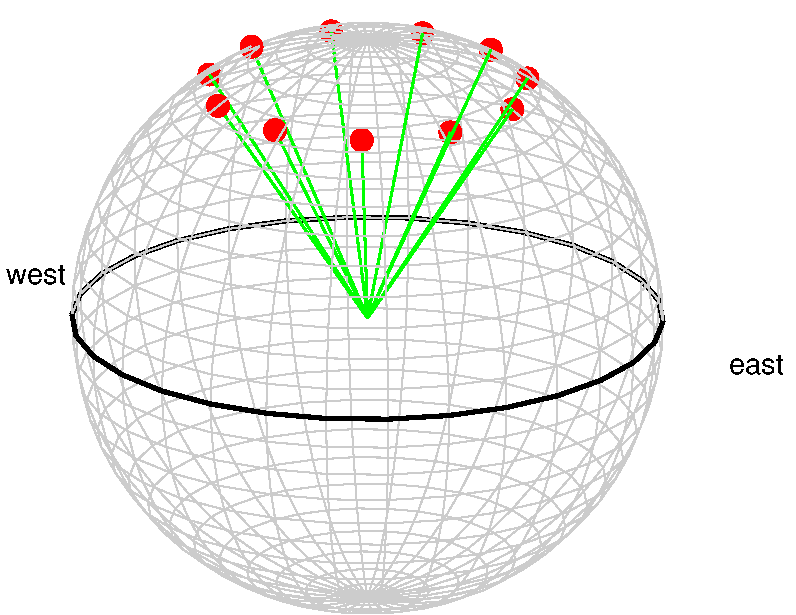
\includegraphics[width=0.45\linewidth]{sota/slant_20.pdf} &
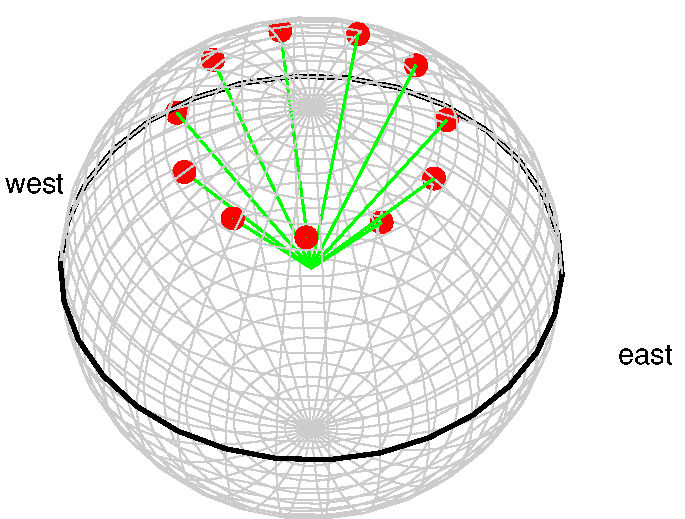
\includegraphics[width=0.45\linewidth]{sota/slant_50.pdf} \\
(a) & (b)
\end{tabular}
\caption{Example of optimal placement using 11 lights, viewed from an elevation of (a) 20\degree and (b) 50\degree. Lights are placed 54.74\degree from the up (zenith) direction. The lights positions are shown in red, the illumination vector are shown in green toward the object to light at the center of the sphere.}
\label{fig:sota-optimalplacement}
\end{figure}

% diffuse light
Contrarily to laboratory conditions, real world lighting is not purely directional. There is always an ambient illumination, also called uniform illumination. This ambient illumination is mainly due to reflections on surfaces like walls and floors and can be far from negligible when a strong light source such as the sun (through a window, for instance) is present. The impact of this ambient illumination on PS was recently looked into~\cite{Angelopoulou2013}. They show surprising results revealing that strong directional light is the most important factor to obtain good reconstruction performance. Useful results can be obtained even when the ambient illumination is up to nine times the strength of the directional lighting, as long as this directional lighting in itself is strong. Weak directional lighting produces bad results, even in the absence of ambient illumination.

% Arbitrary light sources
Research on indoors illumination made a big leap when generic lighting conditions were estimated alongside traditional PS~\cite{basri-ijcv-2007}. This work considered the illumination as a complete sphere around the scene instead of a sum of discrete point light sources. The lighting conditions recovered are, however, limited to low-frequencies. While it can be quite enough for simple materials, it won't work for materials exhibiting specularities or yielding non-Lambertian reflectance.

Pushing the idea of limited lighting directions to its limit gives the two-source PS problem~\cite{hernandez-pami-11}. In this case, a degree of freedom is missing for the normal recovery, giving a single direction where the normal gradient is unknown. This case is interesting in the case of shadowed images, where unconstrained regions can be recovered by propagating surface normal information from around the shadow region. Assuming a smooth object, it is possible to add regularization to the problem to ensure a smooth normal variation over shadowed regions.

%Covering the vast amount of work done on PS as a whole is beyond the scope of this thesis proposal. The rest of the document will focus more closely on work that have considered PS on outdoor conditions.


\section{Outdoor Photometric Stereo}

% webcams
To tackle the new challenge that posed outdoor PS, a natural first strategy has been to experiment with Lambertian reflectance and to model the sun as a point light source, to match a well-studied lab condition. Unfortunately, approaches based on this model have practical limitations caused by the movement of the sun in the sky for a given day. Depending on the latitude and time of year, its trajectory may lie too close to a plane, yielding an under-constrained, two-source PS problem over the whole scene.

\subsection{Using months of data}
\label{sota:ops-months}

The first method that was proposed to make outdoor PS work is to capture several months of data~\cite{ackermann-cvpr-12,abrams-eccv-12} to ensure a good conditioning of the problem. This allows the lighting vectors to spread more, as is shown on fig.~\ref{fig:abrams-sunpath}. Both these work aim to take advantage of online image collections, more precisely webcam timelapses, already available (e.g., WILD~\cite{narasimhan-eccv-06} and AMOS~\cite{jacobs-cvpr-2007}).

\begin{figure}
\centering
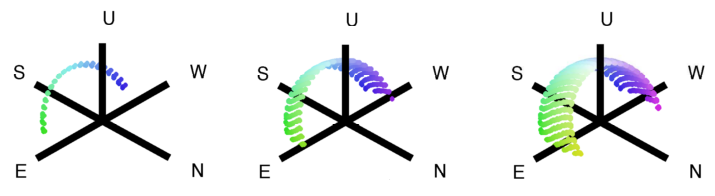
\includegraphics[width=0.8\linewidth]{sota/fig_2b.png}
\caption{Input solar lighting direction on a camera using 1 month, 3 months and 6 months (from left to right). Points are color-coded based on their coordinates: red for north, green for east and blue to make the color a unit-length vector ($b = \sqrt{1 - r - g}$). Figure from~\cite{abrams-eccv-12}.}
\label{fig:abrams-sunpath}
\end{figure}

% Explain Ackermann
A quick overview of the full PS pipeline of~\cite{ackermann-cvpr-12} is now presented. They propose a PS reconstruction algorithm working on webcam timelapses. Their algorithm is divided in three major steps: 
\begin{enumerate}
  \item Selection: choosing the images that should be kept to perform PS, discarding outliers and bad images;
  \item Calibration: performing image subpixel alignment;
  \item PS iterative optimization: optimizing the surface normals and the surface reflectance alternatively.
\end{enumerate}% Selection
First, a selection is made from all the images of the sequence spanning many months. In their analysis, they considered intervals of 6 months or more of data, amounting to a large quantity of images. The selection work is twofold, as they must detect and remove the outliers amongst the images, and then select the best images among the remaining ones. First, they remove images having more than 10\% of their pixels in highlights and mostly dark images, taking care of the outliers. They found that input images with low contrast were harmful for their PS algorithm. As such, to select the best images, they define a contrast measure using the gradient of the object and the portion of the sky visible in the image separately. When strong gradients are found on the object, this means that a strong directional light illuminates the scene, giving a typically interesting input image. They also measure some characteristics of the sky, such as its color, to infer the lighting quality of the image. They suppose that if the visible sky in the image is mostly blue, there is a high risk of the sun shining directly on the object to be reconstructed. These images are good, because a strong directional lighting is what makes PS work. They then blend these two measures together for each image, allowing them to select the best to perform PS on.

% Calibration
Once the best images are chosen, they perform the image alignment. Because mostly of the wind, cameras can move substantially over few months, even when firmly set. In order to work, PS requires an single static viewpoint. Using unaligned images, even so slightly, can have a dramatic performance impact on the reconstruction. To fix this issue, the authors performs a subpixel alignment method (also called image registration) on the input images. Outdoor images can have a very wide variety of illumination condition over the course of many months, making the image registration somewhat problematic. Usually, image registration is done by searching similar zones between two images. But two images lit by two largely different natural illumination conditions will be so different, especially in terms of contrast, that most common image registration algorithms fails in this case. To overcome this problem, they propose to align the images' gradient. To summarize, they use the mean of all the previous image gradients to register a new image. After registration, this new image is embedded into the mean gradient image. A prior art subpixel registration method is employed on these gradient images to perform this step. An example of the alignment distances and mean image is shown in fig.~\ref{fig:ackermann-alignment}.

\begin{figure}
\centering
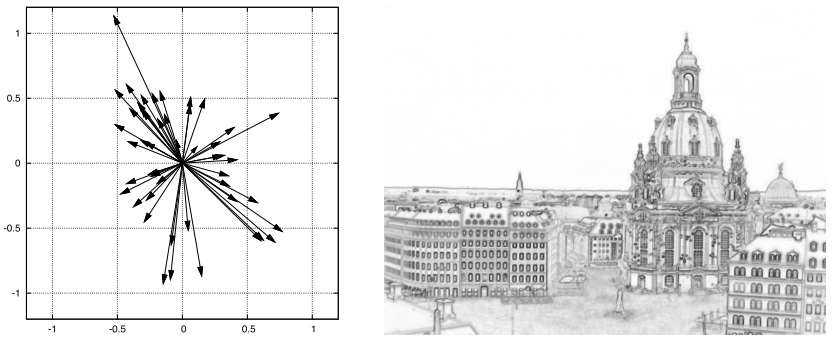
\includegraphics[width=\linewidth]{sota/fig_4.png}
\caption{Motion vectors for image alignment (left): Each arrow corresponds to an image that has been aligned along the direction of its arrow. The axes show the distance of the alignment in pixels. One can see that alignment is very subtle, barely more than a single pixel. The average gradient is shown on the right. Figure and caption from~\cite{ackermann-cvpr-12}.}
\label{fig:ackermann-alignment}
\end{figure}

Then, a radiometric and photometric calibration is performed to recover the response curve of the camera. In most recent PS algorithms, such as this one, this calibration is made by prior art and won't be the main focus of this thesis. It is however important to point out that this calibration is what ensures the image pixels values can be related to a radiance power, allowing the comparison to a light vector.

Afterwards, they employ the method of~\cite{lalonde-ijcv-10} to find the camera azimuth and zenith angles. With this information, the time of day and the approximate GPS coordinates, it is possible to get the sun position with respect to the camera. This gives the light direction needed to perform PS.

The last step of their calibration is an important part of PS in general: shadow detection. Pixels in shadows should be detected and treated differently because they can mess the PS reconstruction. The technique they use first detects when a given pixel is in shadow in every image of the sequence, i.e.\ if all the pixels at the same coordinates in every image of the sequence are in shadow. This first step is quite simple: if the intensity ratio between the maximum intensity and the lowest is less than 1.4, this pixel coordinate is treated to be always in shadow. For every other pixel, they compute the median value $m_\mathrm{min}$ of the $n$ smallest intensity values. A pixel $p$ is flagged as shadowed in image $i$ if its intensity $I_{i,p}$ is smaller than $K \cdot m_\mathrm{min}$. In their case, they chose $n = 10\%$ and $K = 1.5$.

% PS iterative optim
Now that all the selection and calibration done, the PS algorithm can be performed. This PS approach supposes two illumination sources for each image. First, the sun is modeled as a distant point light source. Second, a sky component is used to model everything not explainable by the sun, such as fog or clouds. This sky component is modeled as a spatially uniform light source. When performing the algorithm, they initialize the sky term to be null and set the sun directions to the estimations made using the GPS coordinates, the date and time and the camera orientation. They also initially suppose the surface to be purely Lambertian.

Once the lighting and the material is initialized, they first solve a classical PS formulation. This gives an initial value for the surface normals. Then, they perform an iterative refinement, where they optimize 1) the light intensity between the sky and the sun, 2) the materials among different reflectance functions and 3) the normals to fit the photometric cues.

There are some differences between this work and the second one proposing to capture many months of data~\cite{abrams-eccv-12}. In the latter, they focus on the optimization formulation instead of a full PS pipeline. Also, they suppose a Lambertian surface instead of retrieving the material as~\cite{ackermann-cvpr-12}. In both work, their algorithm is performed independently for each channel of the images (red, green and blue).

Interestingly, \cite{abrams-eccv-12} reported issues on the shadow detection method used by~\cite{ackermann-cvpr-12}. They report that over the span of a year, pixel intensities varies too drastically to have a single correct threshold throughout the sequence. For example, a shadowed pixel when the sun is highest in the sky can have the same intensity as a directly-lit pixel at the opposite time of the year. They thus modify the shadow detection method to be adaptive over time, updating the threshold compared to the previous images analyzed.

Since both techniques are not aware beforehand of the lighting intensities nor the surface albedo, they are subject to the GBR ambiguity. Both work use different techniques to overcome this issue. \cite{abrams-eccv-12} proposes to lift the ambiguity by fixing the exposures to 255 and scaling the rest of their optimization terms accordingly. On the other hand, \cite{ackermann-cvpr-12} proposes to instead cluster the pixels according to their albedo and normals using a machine-learning approach. They find 6 pixels of different normal orientation but seemingly similar albedos, which they use to solve the ambiguity.

While these methods works pretty well, they need data that spans over 6 months, which can be quite cumbersome to acquire. In order to do it in a single day, some modifications to the approach will be needed.

\subsection{Single day}
% single day
Recently, Shen~{\em et al.}~\cite{shen-pg-14} showed that, contrary to common belief, the sun path in the sky actually does not always lie within a perfect plane. Thus, PS reconstruction can sometimes be computed in a single day even with a point light source model. The main downside of this approach is that planarity of the sun path (\ie, conditioning of PS reconstruction) depends on the latitude and the time of year. More specifically, reconstruction becomes unstable at high latitudes near the winter solstice, and worldwide near the equinoxes.

% richer lighting models
To compensate for limited sun motion, a promising approach is to use richer models of illumination that account for additional atmospheric factors in the sky. Typically, more elaborate models of illumination is done by employing (hemi-)spherical high dynamic range (HDR) environment maps~\cite{debevec-siggraph-98,reinhard-book-05} as input to outdoor PS. Encouraging results have been reported in~\cite{yu-iccp-13} for outdoor images taken within an interval of just eight hours (in a single day). Full environment maps can be captured alongside the object captures and used with calibrated PS algorithms~\cite{yu-iccp-13,shi-3dv-14,hung-wacv-15}.

An interesting idea is used by~\cite{yu-iccp-13} to make its algorithm more robust to surface reflectance. They remove the albedo $\rho$ from the original PS equation by dividing an image by another one. First, they find what they call a ``denominator image'', an image yielding as little highlights and shadows as possible. Then, they perform a pixelwise division of every image at time $t$ in the sequence by this denominator image $d$, is represented as
\begin{equation}
\frac{b_{p,i}}{b_{p,d}} = \frac{\rho_p \mathbf{l}_t^T \mathbf{n}_p}{\rho_p \mathbf{l}_d^T \mathbf{n}_p} \quad,
\end{equation}
for pixel $p$. The albedo $\rho_t$ cancels out, giving the relation
\begin{equation}
\left( b_{p,i} \mathbf{l}_d - b_{p,d} \mathbf{l}_t \right)^T \mathbf{n}_p = 0  \quad.
\end{equation}
When using this method, though, we are left with a sequence of 1 image less than to begin with, as dividing an image by itself won't give useful information.

An important note is also made by the authors of~\cite{yu-iccp-13}. When an initial normal map is found, each of these normals defines a new hemisphere of visibility, giving slightly different lighting directions than that was used to compute the initial normal map. It is then possible to perform once again the normal computation using these new lighting directions, leading to an iterative refinement algorithm.

Two algorithm details are also worth noting from this paper: the preprocessing and the regularization. First, they preprocess the images to remove most highlights and shadows. They do so by computing a low-rank matrix minimization of the observed pixel intensity. Because of noise, specularities, shadows and other outliers, the rank of the matrix is higher than 3. By minimizing the rank of the matrix to 3, they eliminate most of these outliers. At the end of the algorithm, they propose to perform a $L_1$-norm regularization called total variation (TV) to increase the accuracy of the reconstruction. This type of regularization promotes sparsity, meaning that few sharp edges should explain better the surface than a low of small normal variations.

While~\cite{yu-iccp-13} dealt with the explicit capture of the environment map, it is also possible to estimate part of the environment map without capturing it, by synthesizing a hemispherical model of the sky using physically-based models~\cite{inose-tcva-13,jung-cvpr-15}.

\cite{inose-tcva-13} employs iterative refinement over the two-source PS approach. Their lighting estimation is done using a white sphere from which they can estimate the parameters of a Preetham model~\cite{preetham-siggraph-99}. While yielding promising results, it requires an object of known shape to be already present in the scene, making it impossible to use with online webcam timelapses. The rest of the method is taken from prior art already explained.

% Jung
% lighting components
\cite{jung-cvpr-15} proposes a fully uncalibrated single day PS reconstruction algorithm. In order to do so, they model the sky into two components: the sky and the sun. These two components are obtain by decomposing the Preetham sky model~\cite{preetham-siggraph-99} into a quadratic skylight and a gaussian sunlight, as shown in fig.~\ref{fig:jung-skysim}. Using this parametric sky model allows for a simple lighting estimation -- with only three variables per component -- and a simple image formation model. As such, a pixel intensity is explained by the superposition of both sky components.

\begin{figure}
\centering
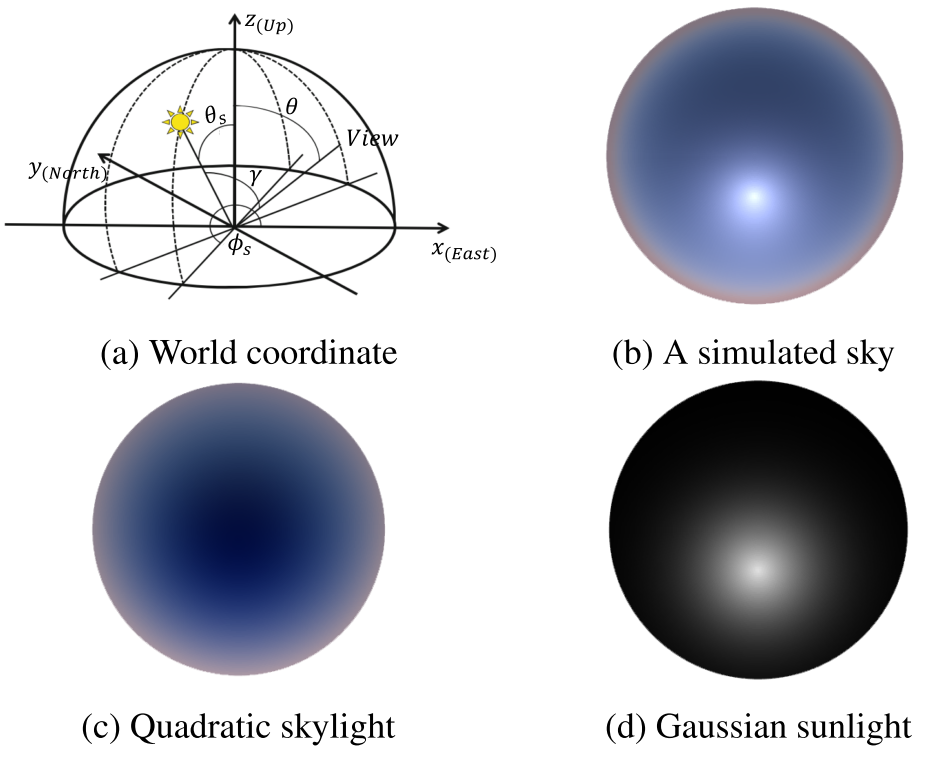
\includegraphics[width=0.5\linewidth]{sota/jung_fig2.png}
\caption{(a) World coordinate specifying the sun position and the viewing direction in the sky hemisphere. (b) A sky hemisphere is simulated using a sky model~\cite{preetham-siggraph-99} and it is parameterized into (c) a quadratic skylight distribution and (d) a Gaussian sunlight distribution. Figure and caption from~\cite{jung-cvpr-15}.}
\label{fig:jung-skysim}
\end{figure}

% color profile and albedo estimation
An interesting yet simple approach for albedo estimation is presented in their work. They report that the color ratio of a pixel throughout the image sequence ($\rho_r : \rho_g : \rho_b$) could be estimated by analyzing the linearity in the color profile. This color profile is the point cloud of a pixel coordinates throughout the image sequence in the RGB cube. The first eigenvector of this point cloud is taken as the relative albedo estimation, which is the dominant direction of the point cloud. Projecting the intensities of the three color channels onto this line gives what they call the pixel profile.

% surface normal sampling
They then perform a coarse surface normal estimation. In order to do so, they sample 1000 points uniformly on a unit sphere and generate the incident irradiance from the skylight and sunlight over the image sequence. Using these, they generate the sample profile, which is an estimated pixel intensity using a sampled normal. Then, the most probable normal is found by taking the highest correlation between these sample profiles and the pixel profiles computed from the images.

% MRF optimization
Using the coarse lighting and normal estimation, the problem is then smoothed and interpolated for shadowed pixels using a Markov Random Field (MRF). This MRF allows a global optimization, solving for the normal that fits best the observations and while taking into considerations its neighbors. It is then possible to inject priors into this optimization. Their neighborhood prior is based on an interesting insight: they remark that pixels yielding similar pixel profiles should have normals close to one another, whereas pixels having different profiles should have mostly orthogonal normals. To formulate this, they use the Pearson correlation coefficient between two neighboring pixel profiles to define how close (or orthogonal) two normals should be.

This algorithm is the current state of the art uncalibrated outdoor single day PS-based approach. The problem is that the reported performance is very far from the performance reported in laboratory conditions. While PS can be taken as ground truth is most laboratory conditions, this algorithm obtains between 30\% and 40\% of the recovered normals under 30\degree of error. This means that 60\% of the recovered normals are outside of a 60\degree cone around the ground truth normal. This amount lowers to 50\% for 4 months of data, which still means that half recovered normals are mostly wrong.




% hold-geoffroy
%The work presented below extends our initial analysis in~\cite{holdgeoffroy-iccp-15}. Rather than presenting a new reconstruction algorithm, in~\cite{holdgeoffroy-iccp-15} we conducted an empirical analysis of the same sky database to identify which days provide more favorable atmospheric conditions for outdoor PS. However, no consideration was given to the shortest time interval of data capture needed to obtain accurate reconstructions; all results were reported on at least 6 hours (a ``full day'') of captured data. Here, instead of comparing days, we focus on analyzing different time intervals within each day. We then show that 6 hours is actually more than necessary, and detail the relationship between the appearance of the sky hemisphere and the quality of PS reconstruction.